% ================= 5. CAD DESIGN =================
\section{CAD Design}
\label{sec:cad}

This design is preliminary: final actuator and sensor specifications are not yet
confirmed, so the mechanical architecture is kept modular and largely
parametric (Section~\ref{sec:background}). This section states the mechanical
concept and the CAD conventions the build follows, for both the first
prototype (the single-face 1-DoF rig) and the second and final prototype (the
three-axis cube), and the checks that confirm the model and the fabricated
parts agree. It is deliberately kept to the level of decisions and interfaces:
the part-by-part model tree, the manufacturing drawings, the fabrication
settings and the assembly sequence are recorded in
Appendix~\ref{app:cad}, so that a change to a bracket does not require an
edit to the design rationale, and the rationale is not buried in geometry.

\subsection{Mechanical Design and CAD Construction}
\label{sec:mechanical}

\subsubsection{CAD Methodology and Model Conventions}
\label{sec:cad_method}

The model is built top-down from the envelope closure of
Section~\ref{sec:massbudget} rather than bottom-up from individual parts, so
that the edge length $L$ and the wheel diameter $D_w$ propagate to every
dependent feature when an iteration changes them. Three conventions make that
propagation reliable, and they are stated here because they constrain how every
part in Appendix~\ref{app:cad} is modelled:

\begin{enumerate}
  \item \textbf{A single skeleton drives the assembly.} $L$, $D_w$, the motor
        axis offsets and the wall thickness live in one parameter table
        referenced by every part; no downstream part carries a hard-coded
        dimension that duplicates one of them.
  \item \textbf{The body frame is the CAD origin.} The assembly origin is the
        cube's geometric centre, with axes on the three motor spin axes, so
        that CAD-reported mass properties are directly the $I$ and $r_{cm}$ of
        Table~\ref{tab:3d_vars} without a change of basis.
  \item \textbf{Mass properties are an output of the model, not an annotation.}
        Every part carries its assigned material and print density, so the
        assembly mass roll-up is the quantity fed back into
        Table~\ref{tab:massbudget} at step~6 of
        Table~\ref{tab:sizing_procedure}.
\end{enumerate}

Convention 3 makes the iteration auditable: the mass budget and the inertia
requirement are read from the same model, so a design that closes analytically
cannot fail to close in the CAD without the discrepancy being detected.

\subsubsection{1-DoF Prototype Build}
\label{sec:cad_2d}

The single-face rig is the first article built and the bench on which the
parameters of Table~\ref{tab:params} are measured. Its structure is a
3D-printed plate sized to one cube face, a central motor and wheel mount, a
corner bearing defining the single rotational degree of freedom, and encoders and other hardware. Note that the servo (brake system) is not included in the 1-DoF prototype as its purpose is validating the control loop on a more well-understood problem. Detailed geometry and the drawing set are in Appendix~\ref{app:cad_2d}.

The rig as built is shown in Figure~\ref{fig:rig_2d}. The plate is mounted
diagonally, so that the pivot bearing sits at the lowest corner and the wheel
axis passes through the plate centre: this places the centre of mass directly
above the contact point at the upright equilibrium, which is the configuration
linearised in Section~\ref{sec:control_algorithms}. The two printed uprights either side
of the frame are hard stops, limiting travel to a few degrees past the point of
no return so that a failed balancing attempt ends against a stop rather than on
the bench.

\begin{figure}[htbp]
\centering
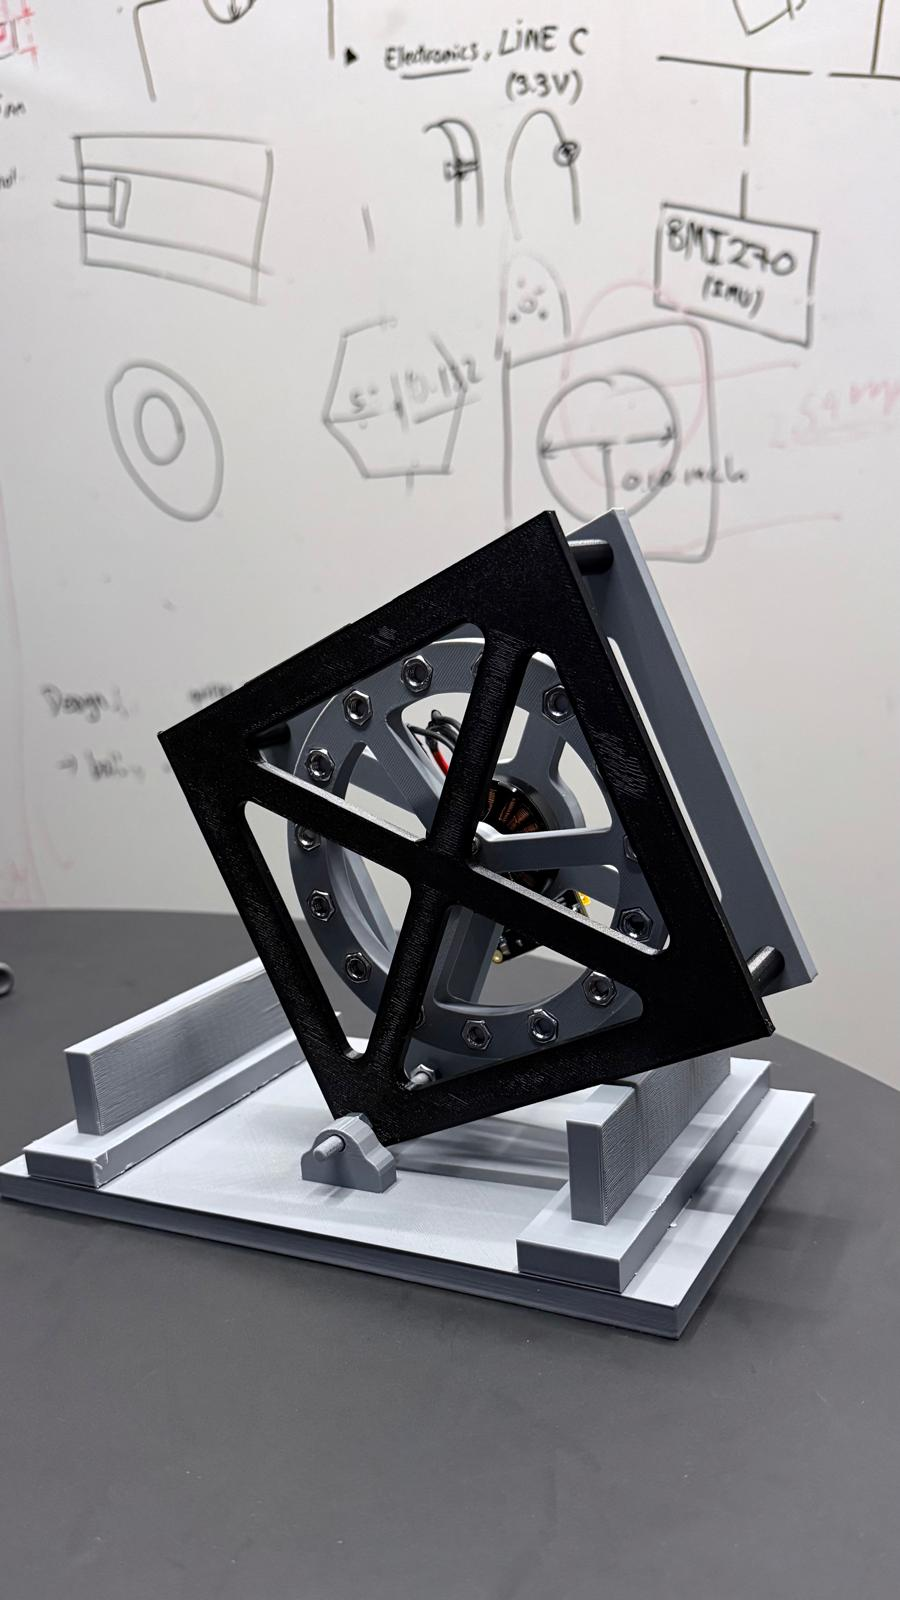
\includegraphics[width=0.52\textwidth]{images/cube_2D.jpeg}
\caption[Single-face (1-DoF) prototype rig as built]{The single-face prototype
rig as built: one reaction wheel driven by a brushless motor on a
diagonally-mounted printed plate, pivoting on a corner bearing against a printed
base with hard stops. This is the article on which the plant parameters of
Table~\ref{tab:params} are measured and the single-axis controller of
Section~\ref{sec:control_algorithms} is validated before the three-axis build. The
drawing set is given in Appendix~\ref{app:cad_2d}.}
\label{fig:rig_2d}
\end{figure}

\subsubsection{3D Cube Frame}

The frame is conceived in two parts, reflecting the constraint chain of
Section~\ref{sec:massbudget}. An \emph{inner structure} locates the three motors
on mutually perpendicular axes through a common centre and carries the battery
pack, the three drivers, the flight controller, inertial measurement unit, and the brake servos; it is the
element that fixes the minimum internal clear volume and therefore the edge
length $L$. An \emph{outer frame} carries the edge and corner contact features,
protects the wheels, and reacts the motor mounting loads from the inner
structure into the ground contact.

A first physical prototype of this frame has been printed and is shown in
Figure~\ref{fig:cube_3d}. It is explicitly a \emph{concept prototype}, not the
flight article: it demonstrates the two-part architecture, the X-braced face
pattern and the packaging of three orthogonal wheel modules within the cube
envelope, and it serves as a physical check on clearances that are awkward to
judge on screen. The final design is not frozen at the time this photograph was taken. Detailed geometry follows
the envelope closure of Section~\ref{sec:massbudget}, and the wheel dimensions
in particular remain open pending the sizing iteration of
Section~\ref{sec:rw_sizing} and confirmation of the final motor; the mass
properties of the printed prototype are therefore not the mass properties
assumed in the budget. The frozen general-assembly drawing is given in
Figure~\ref{fig:dwg_3d} of Appendix~\ref{app:cad_3d}.

The split is also the main mechanical interface in the machine, and it is
managed as one: the inner structure is designed against a fixed bolt pattern and
keep-out envelope published to the outer frame, so the two can be revised
independently as long as that interface holds. The controlled interfaces are
listed in Table~\ref{tab:mech_interfaces}; the parts realising them, with their
drawings, are in Appendix~\ref{app:cad_3d}.

\begin{table}[htbp]
\centering
\caption[Controlled mechanical interfaces]{Controlled mechanical interfaces. Each is frozen once agreed, so that
the parts on either side can be revised independently.}
\label{tab:mech_interfaces}
\small
\begin{tabular}{L{3.6cm} L{3.6cm} L{6.0cm}}
\toprule
Interface & Between & Controlled quantities \\
\midrule
Motor mount        & Motor $\leftrightarrow$ inner structure & Bolt circle, shaft height, concentricity to the wheel axis \\
Wheel hub          & Wheel $\leftrightarrow$ motor rotor     & Bore, bolt pattern, axial location, balance datum \\
Frame joint        & Inner structure $\leftrightarrow$ outer frame & Bolt pattern, keep-out envelope, load path to the contact features \\
Electronics mount  & Board $\leftrightarrow$ inner structure & Board outline, mounting-hole pattern, keep-out heights, connector exit directions (Sec.~\ref{sec:layout}) \\
Brake mount        & Servo $\leftrightarrow$ inner structure & Servo location, barrier throw \\
Battery retention  & Pack $\leftrightarrow$ inner structure & Pack envelope, retention method, centring tolerance to the cube centre \\
Contact features   & Outer frame $\leftrightarrow$ ground    & Corner and edge geometry, material, replaceability \\
\bottomrule
\end{tabular}
\end{table}

\begin{figure}[htbp]
\centering
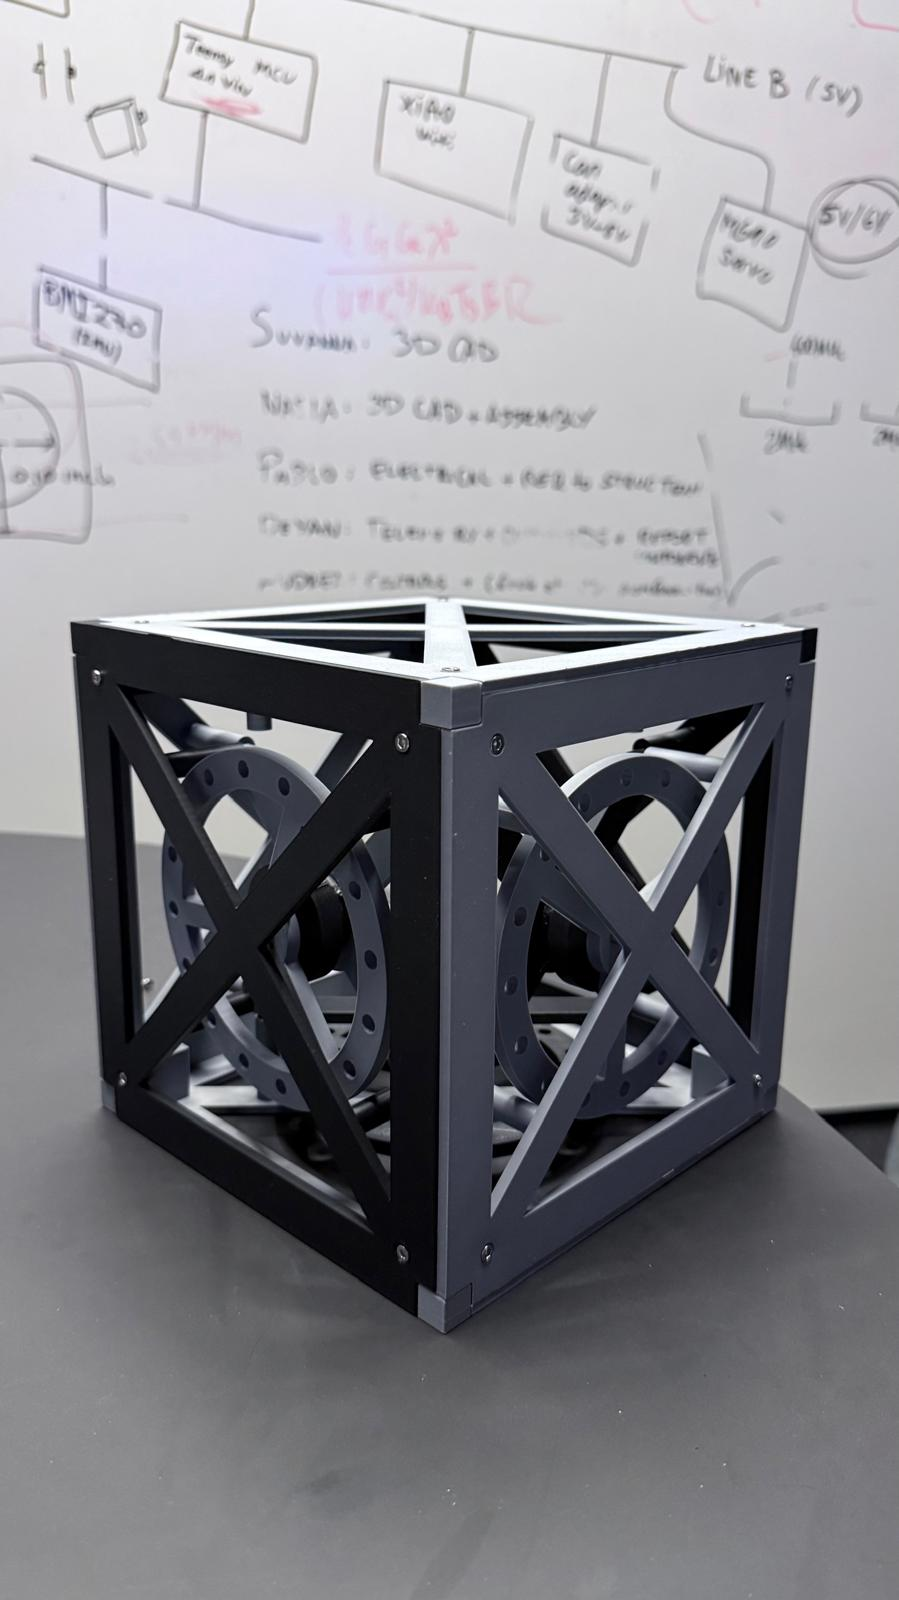
\includegraphics[width=0.48\textwidth]{images/cube_3D.jpeg}
\caption[Printed concept prototype of the three-axis cube frame]{Printed concept
prototype of the three-axis cube frame, showing the X-braced outer faces and the
three orthogonal reaction-wheel modules carried by the inner structure. This
article validates the two-part architecture and the internal packaging only: it
is \emph{not} the final design. Wheel geometry and the frame edge length $L$
remain subject to the sizing closure of Sections~\ref{sec:massbudget}
and~\ref{sec:rw_sizing}, so its mass properties do not represent the budgeted
values. The frozen design's general-assembly drawing is given in
Figure~\ref{fig:dwg_3d} of Appendix~\ref{app:cad_3d}.}
\label{fig:cube_3d}
\end{figure}

\subsection{CAD and Dimensional Verification}
\label{sec:cad_verification}

The checks below split into those that run against the model, before anything is
fabricated, and those that run against the physical part afterwards. The driving
dimensions themselves are outputs of the packaging closure of
Section~\ref{sec:massbudget} and are not verified here; what is verified is that
the model realises them consistently and that the fabricated part matches the
model.

\paragraph{Model checks (pre-fabrication).} Interference and clearance
verification on the wheel-to-subframe and inter-module clearances $c_w$ and $c_o$
of Table~\ref{tab:cad_params}, through a full rotation of each wheel and across
all three axes simultaneously; orthogonality of the three motor axes; position of
the centre of mass relative to the geometric centre, since the modelling of
Section~\ref{sec:methodology} assumes a known offset; and the mass roll-up against
Table~\ref{tab:massbudget}, which is the input to the sizing verification
and must be re-run whenever it changes.

\paragraph{Part checks (post-fabrication).} Dimensional acceptance of the ballast
holes --- diameter, pitch circle radius and the radial wall left on each side ---
since these are structural features rather than cosmetic ones and a print that is
dimensionally out of tolerance at a hole is a wheel that cannot be trusted at
speed; verification that each bolt is torqued and its nyloc nut engaged, the
through-bolt being the retention feature; measured wheel mass against the CAD
prediction; and static balance of the assembled wheel, which is the first
opportunity to detect a ballast placement error before it appears as vibration at
speed.

The modelled-versus-measured comparison is recorded in
Table~\ref{tab:mass_verification} of Appendix~\ref{app:cad_mass} and is not
duplicated here. A discrepancy found at that step is carried back into
$I_{w,\text{target}}$ and absorbed by ballast trim where the authority allows;
where it does not, the finding returns to
the closure procedure rather than being accepted.
